\documentclass[11pt,english,a4paper] {report}
\usepackage[latin1]{inputenc}
\usepackage[T1]{fontenc}
\usepackage{babel,graphicx,varioref}
\usepackage{palatino}
\usepackage{relsize}
\usepackage{varioref}
\usepackage{pdfpages}
\usepackage{fancyvrb}
\usepackage{fancyhdr}
\usepackage{sectsty}
\usepackage{times}
\usepackage{hyperref}
\usepackage{amsmath}
\usepackage{geometry}

%For code listings
\usepackage{color}
\usepackage{xcolor}
\usepackage{listings}
\usepackage{courier}
\usepackage{pdfpages}
\usepackage{varioref}

\definecolor{codegreen}{rgb}{0,0.6,0}
\definecolor{codegray}{rgb}{0.5,0.5,0.5}
\definecolor{codepurple}{rgb}{0.58,0,0.82}
\definecolor{backcolour}{rgb}{0.95,0.95,0.92}
\definecolor{keywordcolor}{RGB}{133,0,3}
\definecolor{commentcolor}{RGB}{135,136,117}
\definecolor{numbercolor}{RGB}{38,38,38}
\definecolor{stringcolor}{RGB}{211,0,53}

%\renewcommand*\rmdefault{Consolas, 'Liberation Mono', Menlo, Courier, monospace}

\def\ff{Consolas, 'Liberation Mono', Menlo, Courier, monospace}

\lstset{
    basicstyle=\scriptsize\fontfamily{\ff},%\footnotesize\ttfamily, % Standardschrift
    numbers=left,               % Ort der Zeilennummern
    numberstyle=\scriptsize,%\tiny,          % Stil der Zeilennummern
    %stepnumber=2,               % Abstand zwischen den Zeilennummern
    numbersep=5pt,              % Abstand der Nummern zum Text
    tabsize=2,                  % Groesse von Tabs
    extendedchars=true,         %
    breaklines=true,            % Zeilen werden Umgebrochen
    %keywordstyle=\color{red},
    frame=b,         
    keywordstyle=[1]\textbf,    % Stil der Keywords
    keywordstyle=[2]\textbf,    %
    keywordstyle=[3]\textbf,    %
    %keywordstyle=[4]\textbf,   \sqrt{\sqrt{}} %
    %stringstyle=\color{white}\ttfamily, % Farbe der String
    showspaces=false,           % Leerzeichen anzeigen ?
    showtabs=false,             % Tabs anzeigen ?
    xleftmargin=17pt,
    framexleftmargin=17pt,
    framexrightmargin=5pt,
    framexbottommargin=4pt,
    %backgroundcolor=\color{lightgray},
    showstringspaces=false,%false      % Leerzeichen in Strings anzeigen ?        
    breakatwhitespace=false,
    keepspaces=true,
    commentstyle=\color{commentcolor}\fontfamily{\ff},%codegreen},
    keywordstyle=\color{keywordcolor}\fontfamily{\ff}, %magenta},
    numberstyle=\tiny\color{numbercolor}\fontfamily{\ff}, %codegray
    stringstyle=\color{stringcolor}\fontfamily{\ff}%codepurple
 }
 \lstloadlanguages{
        Python,
        Bash
 }
    %\DeclareCaptionFont{blue}{\color{blue}} 

  %\captionsetup[lstlisting]{singlelinecheck=false, labelfont={blue}, textfont={blue}}
  %\usepackage{caption}
%\DeclareCaptionFont{white}{\color{white}}
%\DeclareCaptionFormat{listing}{\colorbox[cmyk]{0.43, 0.35, 0.35,0.01}{\parbox{\textwidth}{\hspace{15pt}#1#2#3}}}
%\captionsetup[lstlisting]{format=listing,labelfont=white,textfont=white, singlelinecheck=false, margin=0pt, font={bf,footnotesize}}
\usepackage{caption}
\DeclareCaptionFont{white}{\color{white}}
\DeclareCaptionFormat{listing}{\colorbox{gray}{\parbox{\textwidth}{#1#2#3}}}
\captionsetup[lstlisting]{format=listing,labelfont=white,textfont=white}
% done code

%\usepackage[colorlinks=true,pdfstartview=FitH, linkcolor=blue, 
            %citecolor=blue, urlcolor=blue,bookmarksopen=true]{hyperref}
\def\course{MS016A}
\def\reportname{Lab Report}
\def\name{Lars Haugan}
\author{Lars Haugan - s171201}
\def\studentnr{s171201}
\def\line{NSA}
\def\school{University of Oslo \\ Oslo and Akershus Univeristy College of Applied Sciences}
\def\semester{Autumn 2014}

\hypersetup
{
        pdftitle={\reportname},
        pdfauthor={\name},
        pdfsubject={\reportname},
        colorlinks=true,
        linkcolor=blue,
        citecolor=black,
        urlcolor=blue,
        pdfstartview=FitH,
        bookmarksopen=true
}

\usepackage{apacite}
\bibliographystyle{apacite}

\parindent=0in
\fvset{frame=single,framesep=3mm,fontfamily=helvetica,fontsize=\scriptsize}

\renewcommand\ttfamily{\small\bf\fontfamily{helvetica}}
\newcommand{\HRule}{\rule{\linewidth}{0.2mm}}

\begin{document}
\begin{titlepage}
    \begin{center}

        \large \line\\
        \large \school\\ \semester\\[0.4cm]
        \HRule\\[1.5cm]
        \name, \studentnr
        \ \\[6.0cm]
        \LARGE\textbf{\course\ - \reportname}

    \end{center}
\end{titlepage}


%\title{  \course\ \reportname } %\\ \name \ - \studentnr }

\allsectionsfont{\sffamily}

\tableofcontents

\chapter{Dynamic cloud-based scaling web services}
\textbf{Keywords: Virtualization, Cloud computing, performance, scripting}

\subsection*{Abstract}

This report takes a look at the implementation of a dynamic setup in cloud-based
web-services that scale with the load. With the load balancer HAProxy and
implemented through OpenStack APIs.

\section{Introduction}

\subsubsection{Problem statement}

The given problem statement in this project was as follows:

\emph{Build a cloud-based web service which is able to adjust the number of
webservers based on the incoming rate of user requests.}

\section{Background}
Cloud computing is becoming more and more popular, and is being implemented
in many parts of the industry \cite{OpenStack:Users}. You can rent resources 
from large providers like Amazon which provides a public cloud infrastructure 
or by building your own cloud infrastructure. This can be done with open source 
tools like OpenStack. There is also a third alternative that is the hybrid cloud,
which enables easy transaction from using both a private cloud and public clouds.\\

Having these cloud infrastructures, make it possible to have services
that scale over multiple locations, and to utilize the resources that are
available. When having spanning clouds we can use this to our advantage 
and create solutions to create more sturdy solutions, that will scale web
services in a more cost efficient way.\\

Web services with many consumers or with a high demand for calculation power
will need to be able to use multiple servers to provide service to the clients.
The number of servers needed is proportionate to the number of visitors and
calculations needed to provide the service. If there is not enough servers to
handle the load, there will a result in long response times or even loss of
service.\\

To handle this we need a way of scaling the number of servers in a way that
will give the expected result for the consumers, but at the same time use the
bare minimum amount needed in able to save money.\\

This will make the basis for this chapter where we will look into a solution to
scale a web service over multiple servers in an OpenStack environment.

\subsection{Cloud solution with OpenStack}
OpenStack is a free open source cloud software, that can be used to provide
infrastructure as a service (IaaS). 
OpenStack proclaims to be one of the fastest growing open source communities in
the world, backed by some of the biggest names in the industry like
RedHat and HP \cite{OpenStack:2014}. It is built up of multiple services
where each is responsible to handle a part of the operation in the cloud. Most
notably of these are nova, which handles the instances it selves and the
communication with the vitalization hypervisor. There are a total of 13
services which handles everything from identities, storage, networking,
orchestration and much more.\\

OpenStack is a viable cloud solution due to the large scale implementation, and
the large community supporting further development. One of the features provided 
and result of the open source software are the APIs that are available. 
\textit{Python-novaclient} implementation that provides almost full integration
with nova. Other implementations for the other OpenStack services are also
available. Since OpenStack are implemented in Python, there has been more work
on these API implementations, than what you might expect from a open source
project. According to \cite{OpenStack:api_comparison} the nova API is
compatible with the implementation from Amazon (AWS). This means that it is
possible to use \textit{python-novaclient} also with AWS. This is powerful when
developing tools that are supposed to work with clouds.

\subsection{HAProxy for load balancing}
HAProxy (High Availability proxy) is a free, very fast and reliable solution offering
high availability, load balancing, and proxying for TCP and HTTP-based applications
\cite{haproxy:2014}. It is used by large sites like Reddit, Stack Overflow and
Twitter \cite{haproxy:they_use_it}. Some of the features it provides in the
latest version is native SSL/TLS termination, which is lacking from most other
freely available load balancers, full HTTP keep-alive, IPv6 support, health
checks and much more \cite{haproxy:2014}. There are other free load balancers
that can be used, such as apache with mod, nginx, pound and varnish. Varnish is
mostly used only for caching and does not support SSL/TLS termination. HAProxy
appears to be a de facto standard when it comes to open source load
balancers.\\

These solutions creates a background for the solution to be created that can
make a service scale in a cloud environment. All this so we can save money, and
serve solutions that will prevail with large amounts of requests.
It is also worth noting that it will not only save the provider money, but
ultimately lower energy usage that could lower the environmental impact of a
service.


\section{Approach}
This study will focus on creating a application that enables scaling of a web 
service in a cloud environment. It will explore the possibility of web scaling
by implementing the posibilities of OpenStack and HAProxy in a Python
application. 
This will make it possible to make an application that is tightly integrated
with both OpenStack and HAProxy and make good use of the tight integration.

\subsection{Setup}

\subsection{OpenStack integration}
OpenStack provides excellent possibilities for integration when programming in
Python. With the use of \textit{python-novaclient} it is possible to do almost
anything you can do with nova through either the CLI or OpenStack Horizon.

It is to be expected that the integration can provide all the needed
functionality of handling the instances. This means that it is possible to
handle the creation of new instances and provide the needed information so that
OpenStack handles the installation of the needed software on the new servers.
This can be done through the usage of cloud-data which is served with a
metadata service provided by OpenStack.

With this the application can scale up completely new instances which is
configured for the service within a short amount of time. When the instances
are no longer needed, the integration can shutdown or delete the instance
altogether.

\subsection{HAProxy integration}

\subsection{Needed data}
% Rate of incomming requests.

% How to scale based on the data

\subsection{Expected data}
% Output of the script

\subsection{How to test}

To be able to scale the web service based on the incomming count of requests,
there are multiple aspects that needs to be implemented. These include the
ability to create/start/stop/destroy instances (read: Virtual machines) and
monitor the number of incomming requests.


* Describe the design of the project
* How the data should look
* How to analyze the data

% Is the type of study explained?
% Are all the experiments explained?
% Are the assumptions explained?
% Are there limitations to the approach which you are aware of (NOT hindsight)?
% Is there an explained connection between the data you want to gather and the
% problem you investigate?

\subsection{Creating a webscaler}

\subsection{Data gathering and testing}

 %What is the claim
 %What to do
 %How do i test
 %Output
 %Optional approaches
 %Calcualtion differences
 %reqs
 %reactive \/ proactive

\section{Result}
 %What happened

\section{Analysis}
 %Look at the data
\begin{figure}[htp]
%\centering
%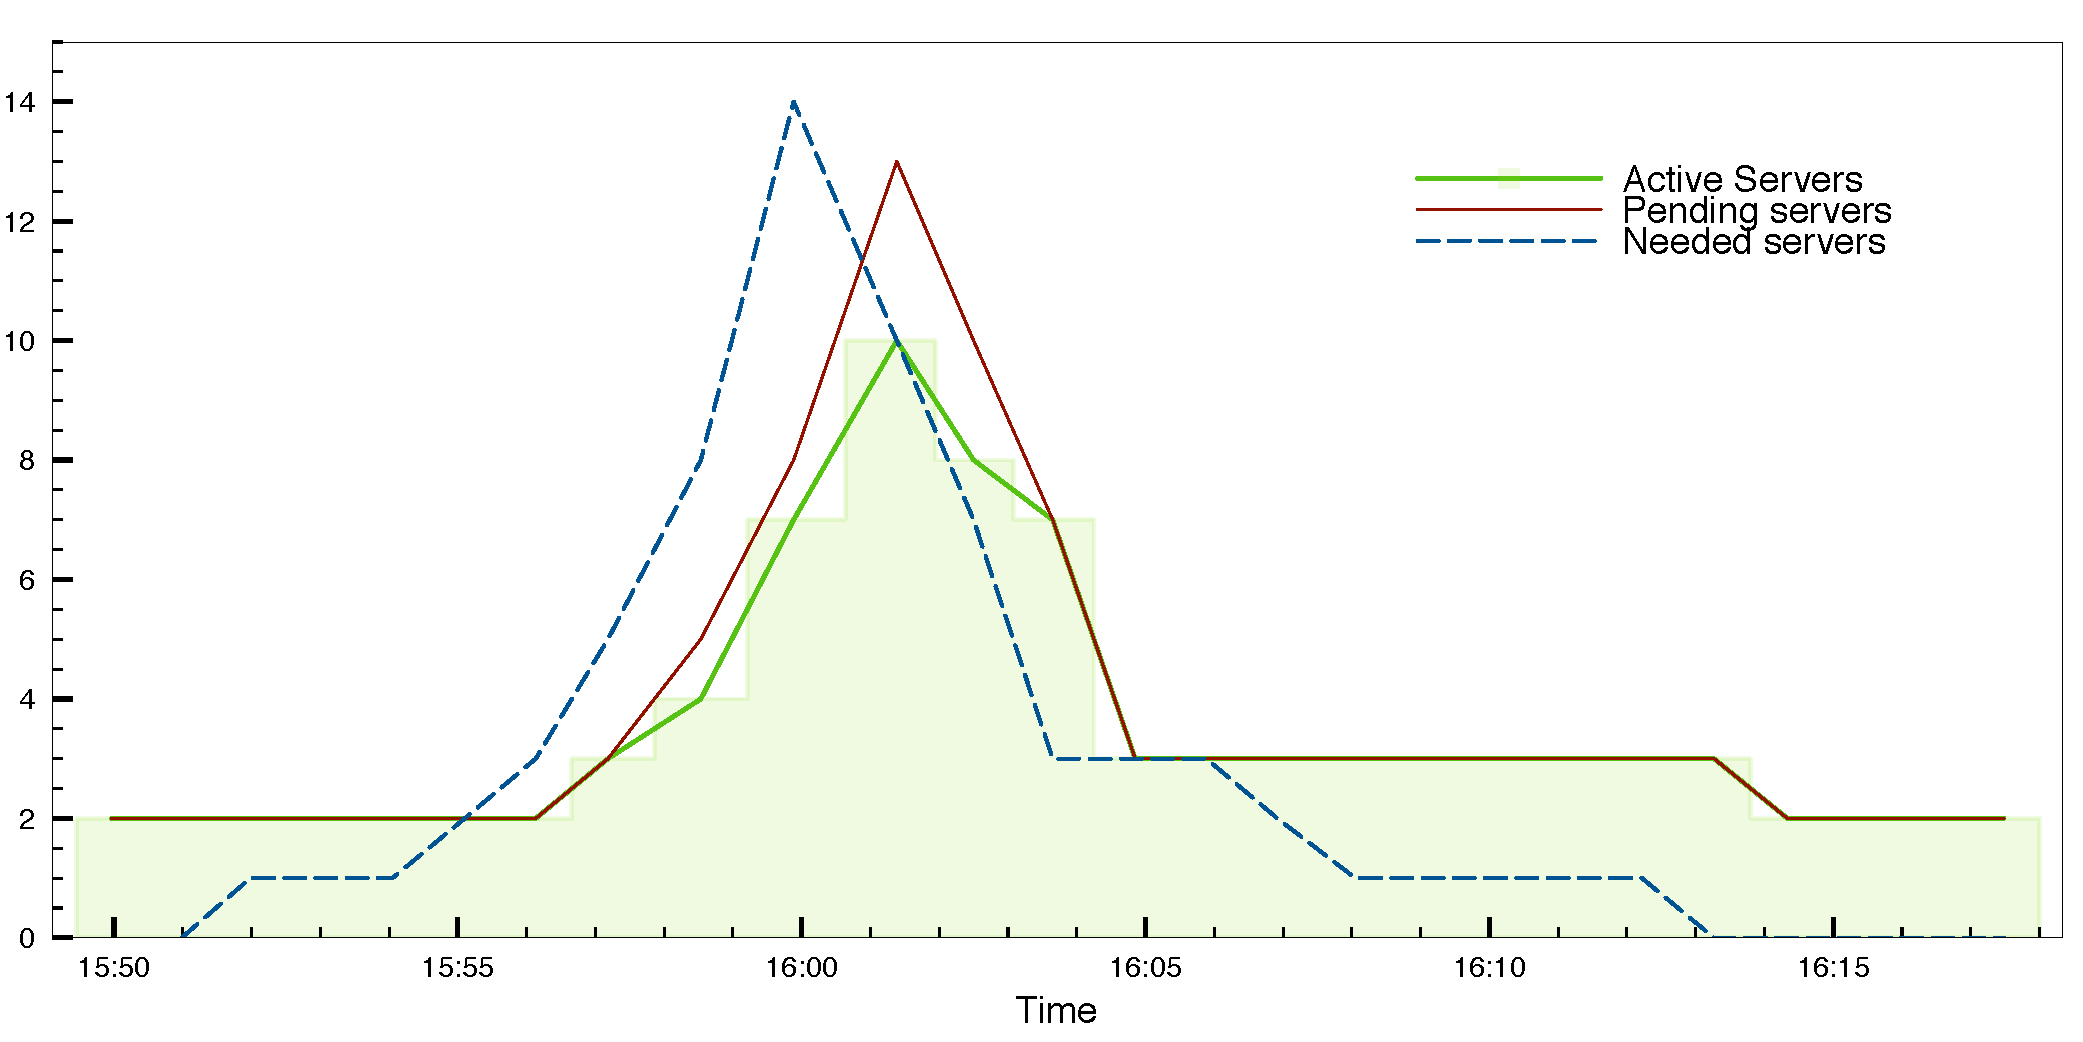
\includegraphics[scale=0.6]{chapter1/server_scaling}
\centering
\makebox[\textwidth][c]{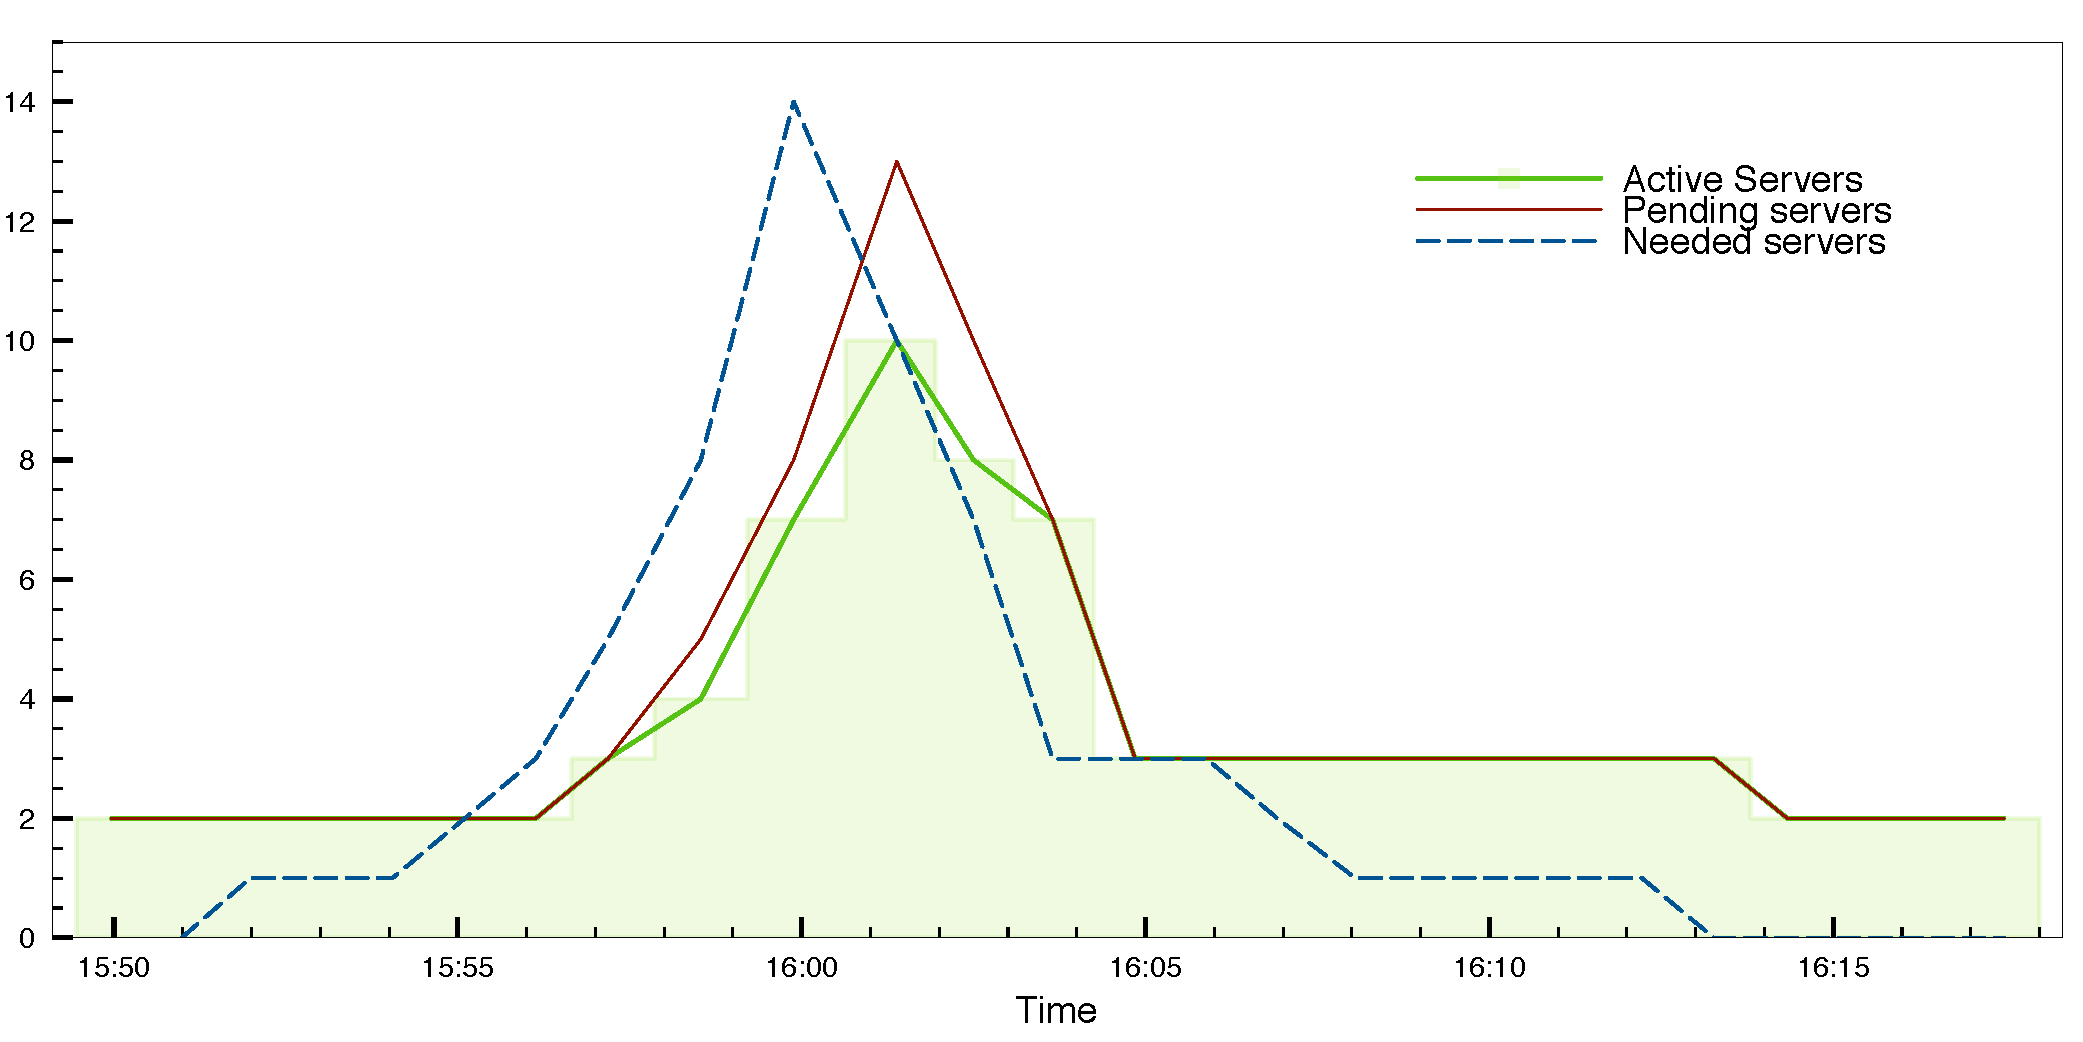
\includegraphics[width=1.2\textwidth]{chapter1/server_scaling}}
\caption{\label{fig:server_scaling}Scaling of servers}
\end{figure}

\section{Discussion and conclusion}
% Why did i not use MLN
\subsection{Improvements}

\subsection{Conclusion}



requests per seconds fornuftig kan vi forvente at en server toler akkurat
det vi har satt i forhold til at det er forskjellige urler



\bibliography{references}

\end{document}
